\documentclass{report}
\usepackage[utf8]{inputenc}
\usepackage[french]{babel}
\usepackage[version=3]{mhchem} % Package for chemical equation typesetting
\usepackage{siunitx} % Provides the \SI{}{} and \si{} command for typesetting SI units
\usepackage{graphicx} % Required for the inclusion of images
\usepackage{natbib} % Required to change bibliography style to APA
\usepackage{amsmath} % Required for some math elements 
\usepackage{wrapfig}
\usepackage[top=2cm,left=2cm,bottom=2cm,right=2cm]{geometry}
\usepackage[table]{xcolor}
\usepackage{float}
\usepackage{mathtools}
%----------------------------------------------------------------------------------------
%	INFORMATION DU DOCUMENT
%----------------------------------------------------------------------------------------

\title{Sorbonne Université\\Compte rendu de travaux pratiques de l'UE \\Apprentissage et Reconnaissances des Formes} % Title
\author{Asma \textsc{BRAZI} 3703554\\} % Author name
\date{Master 1 ANDROIDE\\ Année universitaire 2018/2019}

%----------------------------------------------------------------------------------------
%	CONTENU DU DOCUMENT
%----------------------------------------------------------------------------------------
\begin{document}
\maketitle

%----------------------------------------------------------------------------------------
%	INTRODUCTION
%----------------------------------------------------------------------------------------
\tableofcontents
\begin{abstract}
Ce rapport a pour objectif de présenter le travail que nous avons effectué, dans le cadre des travaux pratiques de l'UE ARF (Apprentissage et Reconnaissance des formes). Notre objectif et d'étudier des méthodes quantitatives en Intelligence Artificielle et en reconnaissance des formes. Nous y rassemblons nos expériences, nos résultats et nos observations. Ce document regroupe les quatre premiers TME où chaque chapitre concerne un TME. 
\end{abstract}

\chapter{Arbres de décision, sélection de modèles}

%----------------------------------------------------------------------------------------
%	ARBRES DE DÉCISION
%----------------------------------------------------------------------------------------



\begin{wrapfigure}{r}{0.2\textwidth}
  \vspace{-20pt}
  \begin{center}
    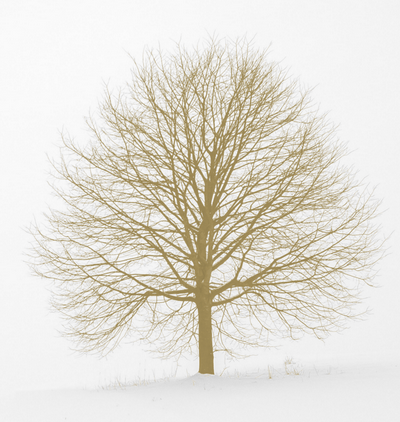
\includegraphics[width=0.2\textwidth]{tree.png}
  \end{center}
  \vspace{-20pt}
  \vspace{-10pt}
\end{wrapfigure}

\paragraph{}
Afin de sélectionner le meilleur attribut à chaque niveau,\\ nous calculons l'entropie de Shannon pour caractériser le degré de désorganisation ou d'imprédictibilité d’un échantillon. \\
Alors, lorsque nous avons un nouvel exemple qui se présente, il sera classé, en le soumettant à une séquence de tests. À la fin de ces tests,la classe à laquelle appartient l'exemple est déterminée. 
\\
\\
\section{Expérience préliminaires sur le modèle}
\paragraph{}
Soit IMDB (Internet Movie DataBase) notre base d'exemples que laquelle notre expérience s'effectue. Pour commencer, nous allons étudier dans cette partie l'impact de la profondeur de l'arbre sur le nombre  d'exemples générés au niveau des feuilles. Pour cela nous allons varier la valeur de la profondeur de l'arbre et voir son impact.
\linebreak
\linebreak
\begin {center}
\begin{tabular}{|c|c|c|c|c|}
  \hline \rowcolor{lightgray}
  Profondeur & 3 & 5 & 10 & 20 \\
  \hline
  Score & 0.71 & 0.73 & 0.82 & 0.89 \\
  \hline
\end{tabular}
\end {center}
\paragraph{}
Tout d'abord, le nombre d'exemples générés croit (resp décroît) lorsque la profondeur de l'arbre augmente (resp diminue). Puis, le score obtenu augmente aussi lorsque nous augmentons la profondeur de l'arbre. Car cette dernière spécialise la classification. En revanche, un score trop élevé limite les capacités de généralisation.

\paragraph{}
 Nous précisions que ces scores ne sont guère un indicateur fiable du comportement de l’algorithme, puisque ces évaluations ont été réalisées sur les données d’apprentissage. Afin d'obtenir un indicateur fiable, nous divisons notre base en deux sous-ensembles. Le premier sous-ensemble correspondrait à l'ensemble d'apprentissage et le second à l'ensemble de test.
 
%----------------------------------------------------------------------------------------
%	SUR SOUS-APPRENTISSAGE
%----------------------------------------------------------------------------------------


\section{Sur et sous apprentissage}
\paragraph{}
Dans cette partie, nous allons effectuer différents partitionnement de l'ensemble initial en un ensemble d'apprentissage et un ensemble de test. À savoir: (0.2, 0.8), (0.5, 0.5) et (0.8, 0.2). Nous traçons les courbes de l'erreur en apprentissage et de l’erreur en test en fonction de la profondeur du
modèle. 

\begin{figure}[H]
  \begin{center}
    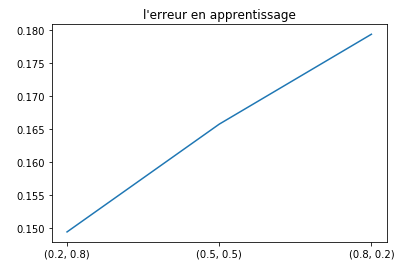
\includegraphics[width=0.4\textwidth]{erreur_app_part.png}
    \caption{Courbe de l’erreur en apprentissage pour différentes partitionnements de l'ensemble des données}
  \end{center}
\end{figure}


\begin{figure}[H]
  \begin{center}
    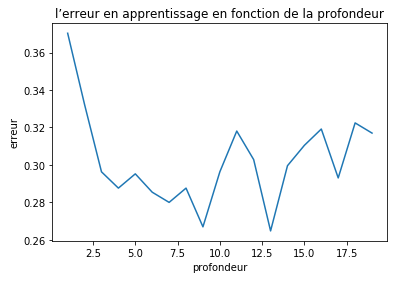
\includegraphics[width=0.4\textwidth]{erreur_app.png}
    \caption{Courbe de l’erreur en apprentissage en fonction de la profondeur de l'arbre}
  \end{center}
\end{figure}

\begin{figure}[H]
	\begin{center}
		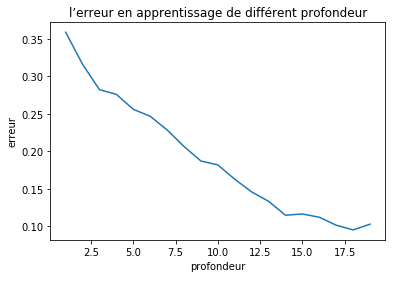
\includegraphics[width=0.4\textwidth]{erreur_test.png}
		\caption{Courbe de l’erreur en test en fonction de la profondeur de l'arbre}
	\end{center}
\end{figure}
\paragraph{}
Quand il y a peu d'exemples d'apprentissage, le score de prédiction est faible car le modèle n'apprend pas suffisamment. D'ailleurs, nous sommes presque dans l'aléatoire. Dans le cas contraire, lorsqu'il y a beaucoup d'exemples d'apprentissage, le modèle sur-apprend et il sera pas très bon à la prédiction car il ne sera pas très bon à la généralisation. Par conséquent, nous obtenons un score faible à la prédiction. D'où une faible performance.

\begin{figure}[H]
  \begin{center}
    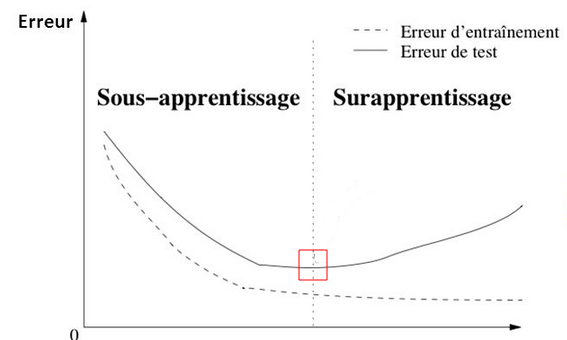
\includegraphics[width=0.4\textwidth]{apprentissage.png}
    \caption{Mémorisation de l'ensemble d'apprentissage}
  \end{center}
\end{figure}
\paragraph{}
Il est inévitable de trouver un compromis entre le sur-apprentissage et le sous-apprentissage, où le modèle est bon sur ces deux ensembles. Sur la figure ci-dessus, le point que nous cherchons à atteindre est encadrer 

\paragraph{}
Comme solution, nous pourrons considérer un ensemble de validation. Ceci reste une méthode simple et efficace. Ce qui permet d'entraîner et de tester le modèle K fois sur différents sous-ensembles et d'estimer la performance sur de nouvelles données.


%----------------------------------------------------------------------------------------
%	VALIDATION CROISÉE
%----------------------------------------------------------------------------------------
\section{Validation croisée}
\paragraph{}
Comme nous espérons obtenir des résultats plus fiables et stables, nous cherchons à utiliser la base initiale de données complètement. Pour cela, la méthode de la validation croisée nous permet de tester à quel point notre modèle est efficace sur un ensemble de validation supposé. Surtout, lorsque nous avons pas un ensemble de validation explicite. La méthode consiste à partitionner notre base de données en N partitions. Puis, nous effectuons N itérations où à chaque tour de boucle, nous considérons la ième partition comme une base de test et les autres partitions restantes comme une base d'apprentissage.

\begin{figure}[H]
  \begin{center}
    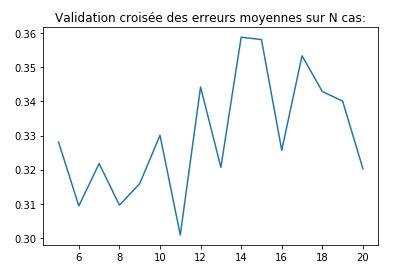
\includegraphics[width=0.5\textwidth]{cross_courbe.png}
    \caption{Courbe des erreurs moyennes sur N cas}
  \end{center}
\end{figure}
\paragraph{}
L'expérience dont les résultats se résument dans la figure ci-dessus nous montre que lorsque la profondeur est égale à 11, nous obtenons les meilleurs résultats.

%----------------------------------------------------------------------------------------
%	ESTIMATION DE DENSITÉ
%----------------------------------------------------------------------------------------
\chapter{Estimation de densité}
\paragraph{}
La densité de probabilité décrit la distribution des données dans l'espace vectoriel. Ceci nous permet une meilleure maîtrise des caractéristiques de ces données, à travers les régions les couvrant.
\paragraph{}
L'étude que nous menons, consiste à estimer la loi de densité géographique des points d'intérêts sur Paris. Plus précisément pour le POI textbf{atm}.Dans le cadre du module, nous étudions deux méthodes d'estimation de densité: la méthode des histogrammes et la méthode à noyaux.

\section{Définition}
\paragraph{}
La méthode des histogrammes représente la répartition des données à l'aide des histogrammes, pour approximer la fonction de densité.
Dans notre étude, nous discrétisons la carte géographique en comptant le nombre d'observations appartement à chaque région. 

\paragraph{}
La méthode à noyaux consiste à retrouver la continuité que nous perdons dans la méthode des histogrammes. En effet, grace au paramètre \textbf{h} que nous fixons, l'estimation peut devenir lisse. Cependant, un exemple proche du point de support \textbf{x} se voit attribué une grande valeur et vis-versa. 
\section{Expérimentations}
\paragraph{}
Nous allons effectuer quelques expériences sur l'estimation de densité par différentes méthodes. Pour commencer, nous allons étudier la méthode des histogrammes en variant la largeur de chaque bin de l'histogramme.

\begin{figure}[H]
	\begin{center}
		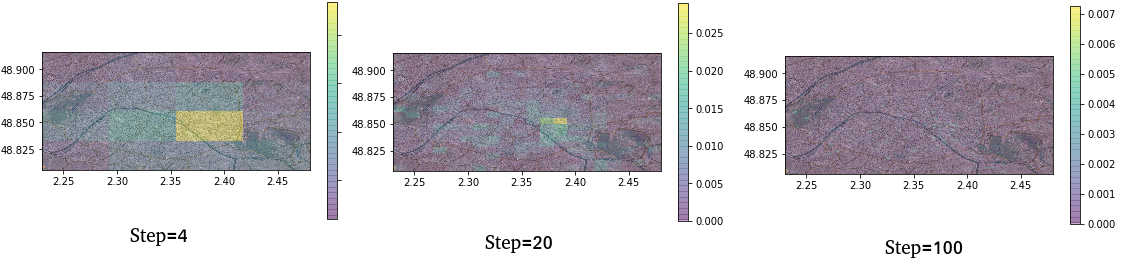
\includegraphics[width=1\textwidth]{histo.png}
		\caption{Estimation de densité par la méthode des histogrammes }
	\end{center}
\end{figure}
\paragraph{}
Nous remarquons que lorsque nous fixons le pas de discrétisation à une grande valeur, la précision devient pointilleuse créant des discontinuités. Cependant, ceci rend le modèle incapable de généraliser.Nous dirons que le modèle sur-apprend. Dans le cas contraire, un faible pas de discrétisation regroupe les données dans de larges bins. Ceci résulte une faible précision. Aussi, Comme ces données ne partagent pas forcément les mêmes caractéristiques, alors  nous nous retrouvons dans un abus de généralisation. Le modèle sous-apprend.
\paragraph{}
Maintenant, nous allons étudier la méthode à noyaux. Les noyaux implémentés sont Parzen et et Gauss.
\begin{figure}[H]
	\begin{center}
		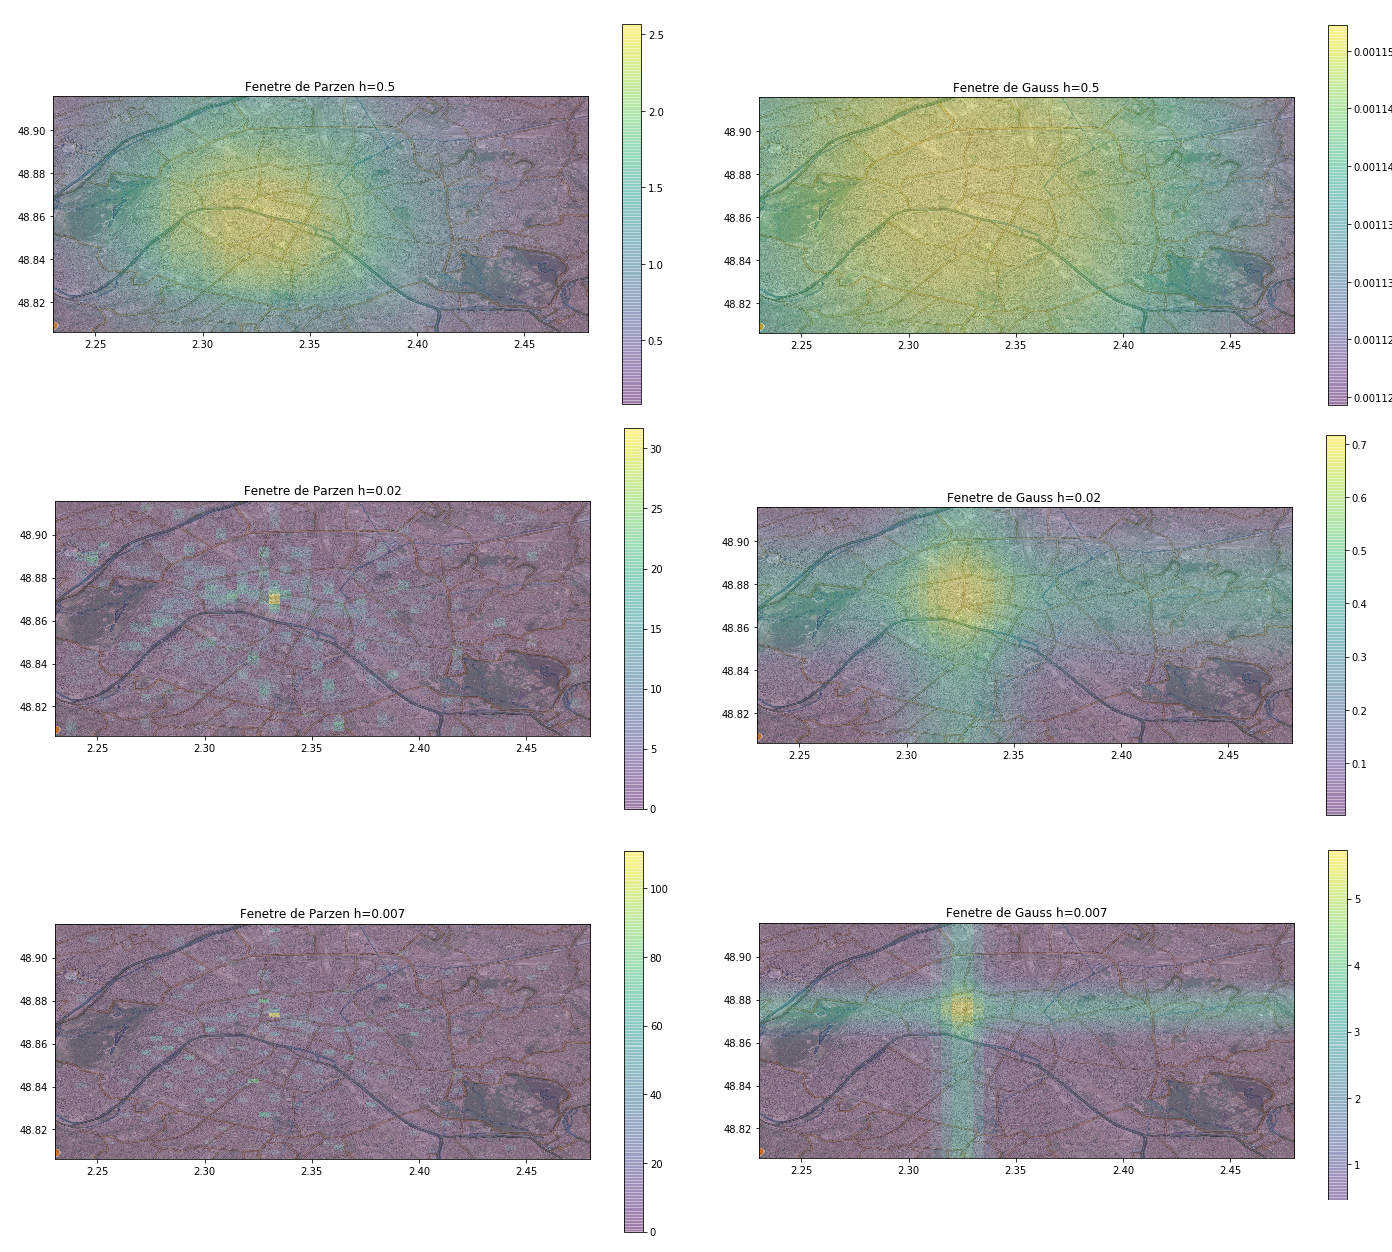
\includegraphics[width=1\textwidth]{parzen_vs_gauss.png}
		\caption{Estimation de densité par la méthode à noyaux (Parzen et Gauss)}
	\end{center}
\end{figure}
\paragraph{}
À la différence de la méthode des histogrammes, la méthode à noyaux considère le voisinage du point courant que l'on souhaite lui approcher sa densité pour éviter la discrétisation. Ce voisinage est déterminé par les paramètres du modèle. Après avoir étudié plusieurs cas de figure en variant le paramètre \textbf{h}. Nous concluons qu'avec une base d'observations importante, il serait nécessaire de fixer un \textbf{h} grand pour un lissage important. 
\subsection{Calcul du paramètre optimal h* de Gauss }
Nous avons utilisé une formule tirée d'un article de recherche\footnote{Les deux chercheurs VIKAS CHANDRAKANT RAYKAR et RAMANI DURAISWAMI ont publié un article intitulé \textbf{Very fast optimal bandwidth selection for univariatekernel density estimation}. Cet article explique le procédé suivi pour approcher la valeur de h optimale.} permettant d'estimer la valeur de h de manière optimale: $h=(4\sigma^5/3n) \approx 1.06\sigma n^(-1/5)$.
\paragraph{}
Approximativement, nous avons trouvé comme valeur de h*=0.11. Avec ce résultat, nous allons refaire les expériences avec la fenêtre de Parzen et le noyau de gauss.
\begin{figure}[H]
	\begin{center}
		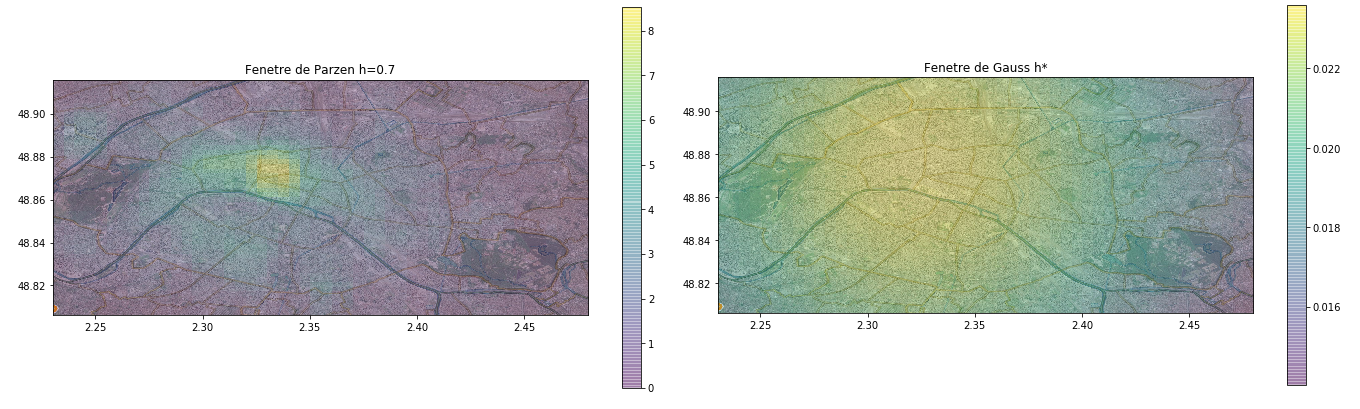
\includegraphics[width=0.8\textwidth]{h*_test.png}
		\caption{Estimation de densité avec h* par la méthode à noyaux (Gauss)}
	\end{center}
\end{figure}
\paragraph{}
Les résultats obtenus pour la fenêtre de Parzen sont plus intéressants par rapport aux résultats que nous avons obtenus précédemment, car dans ces résultats nous pouvons voir mieux la répartition des données et où elles sont denses. Pour le noyau de Gauss, nous avons obtenu des résultats se rapprochant des résultats obtenus à la section précédente. 
\chapter{Descente de gradient}
\section{Optimisation de fonctions}
\paragraph{}
Nous avons implémenté trois fonctions ci-dessous afin d'essayer de chercher une valeur qui minimise une fonction donnée. Pour ce faire, nous utilisons la descente de gradient qui nous permet de générer une suite de valeurs $ x_{i} $ , partant d'un point initial aléatoire et espérer arriver au point minimisant cette fonction. Il est possible que l'algorithme ne converge pas pour certaines raisons que nous citerons plus tard dans le rapport. Donc, nous utilisons un nombre maximum d'itérations et aussi un pas d'apprentissage.

\begin{align}
f(x) &= x \cos{x}
\end{align}
\begin{align}
f(x) &= -\log{x}+x^2
\end{align}
\begin{align}
f(x_1,x_2) &= 100(x_1-x_2^2)^2+(1-x_1)^2
\end{align}
\subsection{Expérimentations}
\paragraph{}
Nous essayons dans cette partie de varier les paramètres de l'algorithme: nombre d'itérations et le pas d'apprentissage et de voir leur impact sur les résultats. Pour chaque exécution donnée de paramètres donnés, nous avons tracé quelques graphes. Une première figure regroupant trois courbes en fonction du nombre d'itérations: l'ensemble des $ x_{i} $, $f(x)$ et $\nabla f(x)$. La deuxième figure explicite la trajectoire. Enfin nous traçons la courbe $ \log(||x^t-x^*||) x_{i} $ qui nous permet de visualiser à chaque itération à quel point nous nous rapprochons de la solution optimale $x^*$.
 
\begin{enumerate}
	\item \textbf{Optimisation de la fonction $f(x)= x\cos(x)$}
	\paragraph{}
Nous démarrons notre optimisation avec $ x_{0}=1 $ avec un nombre d'itérations $n=50$ et un pas d'apprentissage $ \epsilon=0.05$. La première figure représente trois courbes, la courbe des $ x_{i} $ nous montre que la valeur point final estimé $x^* \approx 3.5$ où d'ailleurs le gradient s'annule. 
La deuxième figure, nous montre la trajectoire dessinée par la série de valeurs  $ x_{i}$ de l'optimisation où nous pouvons bien constater que nous démarrons avec $ x_{0}=1 $. Nous notons que la série de valeurs  $ x_{i}$ converge vers le minimum de la fonction.
 \begin{figure}[H]
 	\begin{center}
 		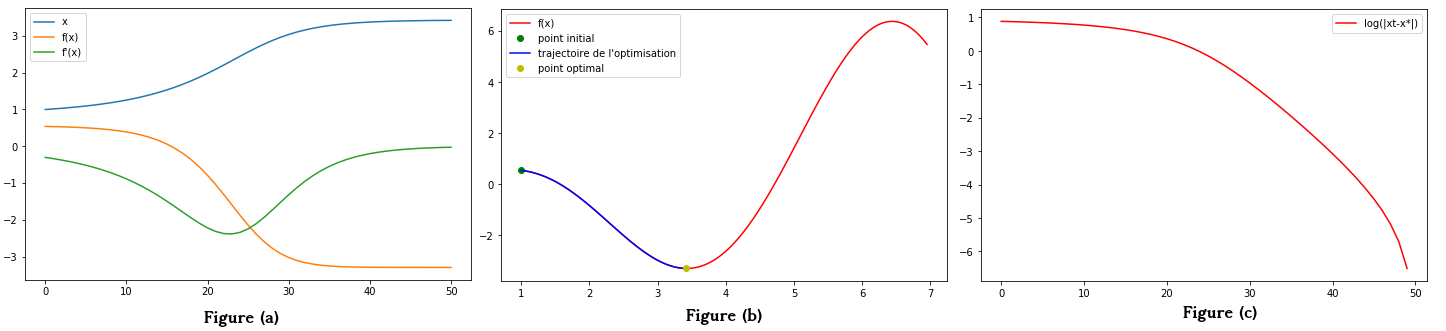
\includegraphics[width=1\textwidth]{f1.png}
 		\caption{Optimisation de la fonction $f(x)= x\cos(x)$ pour $\epsilon=0.05$ et le nombre d'itération=50}
 	\end{center}
 \end{figure}
\paragraph{}
Si nous démarrons notre descente avec une autre valeur initiale soit $ x_{0}=7 $. Nous obtenons un autre optimum (optimum global dans ce cas). Nous pouvons voir dans la figure ci-dessous que la valeur optimale obtenue dans l'expérience précédente n'est qu'un optimum local. Par conséquent, le résultat obtenu dépend de la valeur initiale choisie et le résultat obtenu n'est pas forcément l'optimum global.
 \begin{figure}[H]
	\begin{center}
		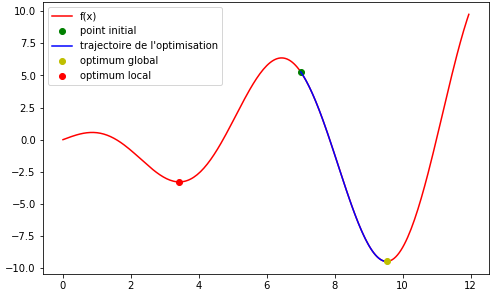
\includegraphics[width=0.4\textwidth]{f1_glob_loc.png}
		\caption{Optimisation de la fonction $f(x)= x\cos(x)$ pour $\epsilon=0.05$ et le nombre d'itération=50}
	\end{center}
\end{figure}
Nous répétons la même expérience mais cette fois-ci nous allons changer la valeur du pas d'apprentissage pour le fixer à $ \epsilon=0.8$. Nous remarquons que l'algorithme ne converge pas vers la solution optimale. Comme le pas d'apprentissage est très grand, nous avons un phénomène d'oscillations qui se crée. De ce fait, l'algorithme n'arrivera pas à atteindre son minimum. 
 \begin{figure}[H]
	\begin{center}
		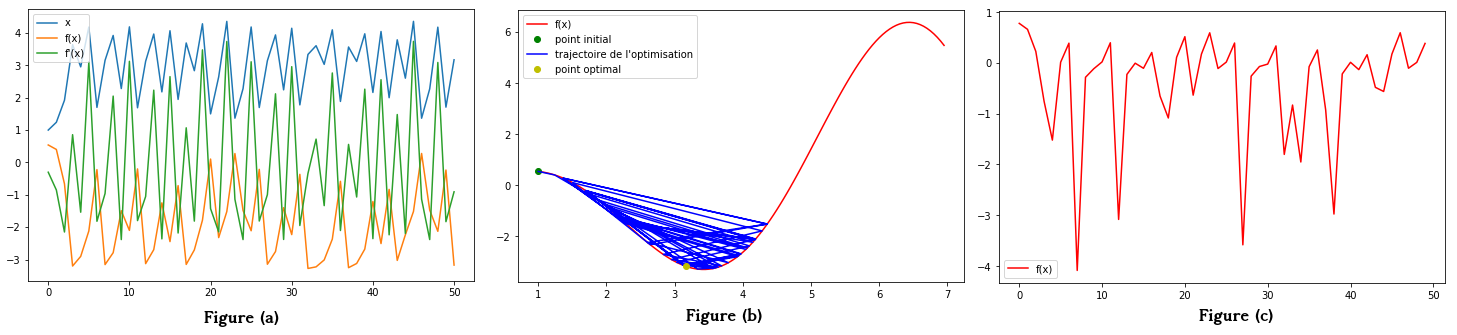
\includegraphics[width=1\textwidth]{f1_epgrand.png}
		\caption{Optimisation de la fonction $f(x)= x\cos(x)$ pour $\epsilon=0.8$ et le nombre d'itération=50}
	\end{center}
\end{figure}
\paragraph{}
Maintenant, nous allons tester la descente de gradient avec un epsilon très petit. Soit $\epsilon=0.001$ avec le nombre d'itération=50.
Malgré le nombre d'itérations augmenté à 50, nous remarquons que l'algorithme prend beaucoup de temps pour passer de $ x=1 $ à $ x \approx 1.1 $ et par conséquent n'atteint pas la valeur optimale. Pour cela, nous avons poussé le nombre d'itérations à 2000. Et là, nous arrivons à atteindre le point optimale.	
 \begin{figure}[H]
	\begin{center}
		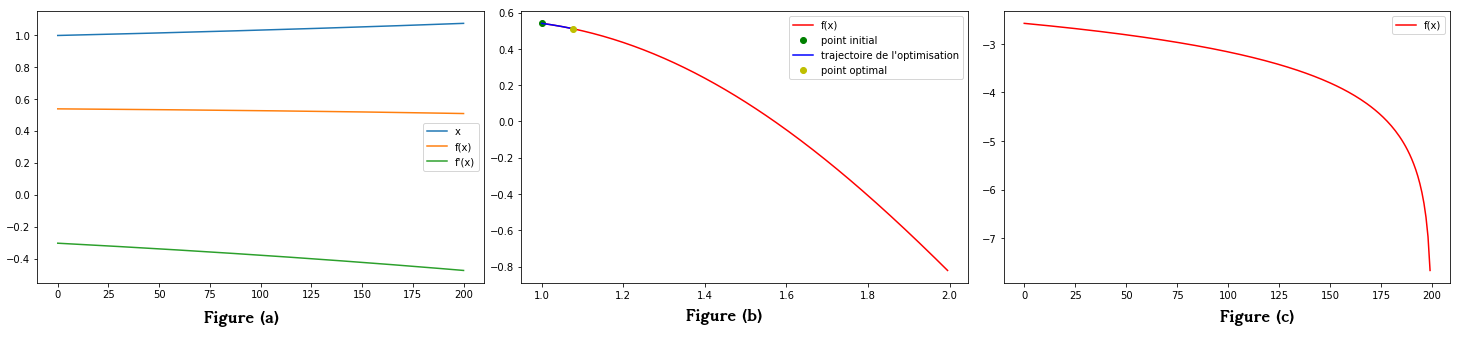
\includegraphics[width=1\textwidth]{f1_eppetit1.png}
		\caption{Optimisation de la fonction $f(x)= x\cos(x)$ pour $\epsilon=0.001$ et le nombre d'itération=200}
	\end{center}
\end{figure}

 \begin{figure}[H]
	\begin{center}
		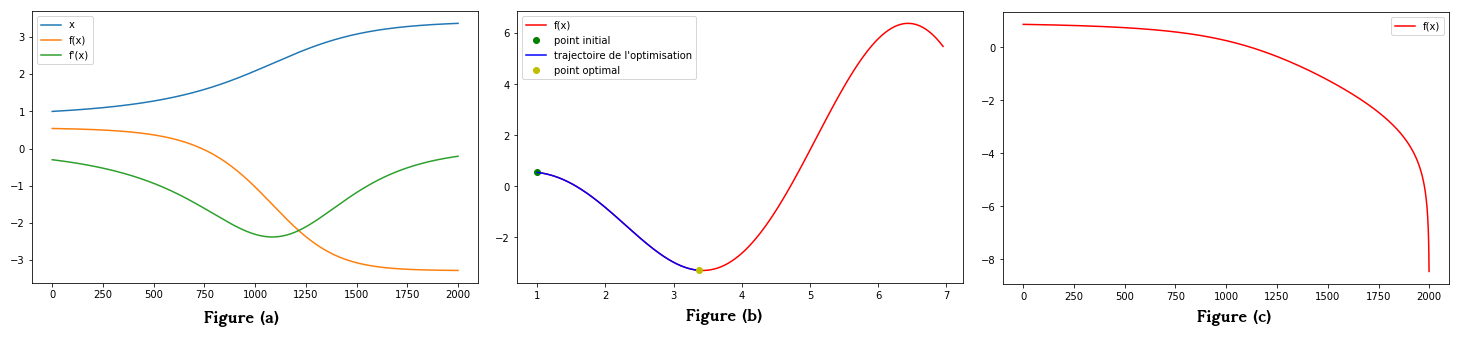
\includegraphics[width=1\textwidth]{f1_eppetit2.png}
		\caption{Optimisation de la fonction $f(x)= x\cos(x)$ pour $\epsilon=0.001$ et le nombre d'itération=2000}
	\end{center}
\end{figure}

\item \textbf{Optimisation de la fonction $f(x)=-\log{x}+x^2$}
\paragraph{}
De la même façon que, nous avons optimisé la fonction $f(x)=-\log{x}+x^2$. En partant avec comme valeur initiale  $ x_{0}=3 $, nous sommes arrivés à la valeur optimale $x \approx 0.7$
\begin{figure}[H]
	\begin{center}
		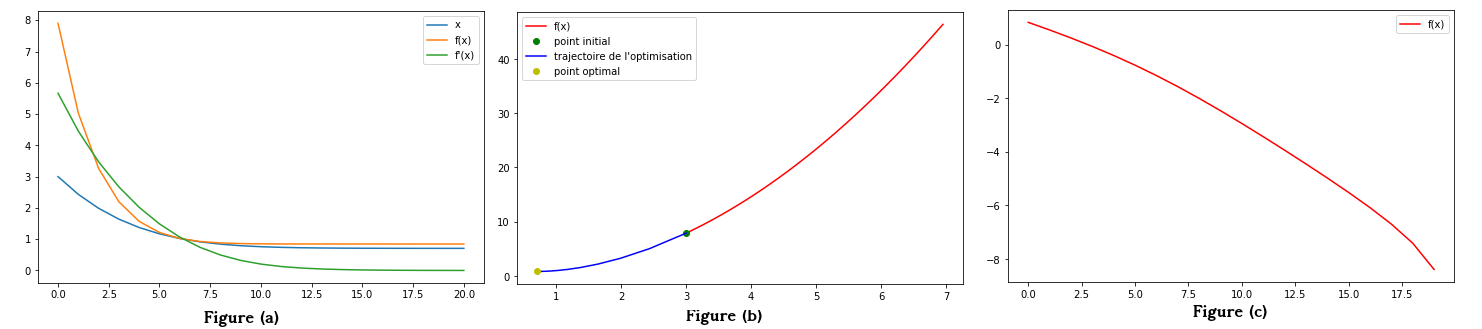
\includegraphics[width=1\textwidth]{f2.png}
		\caption{Optimisation de la fonction $f(x)=-\log{x}+x^2$ pour $\epsilon=0.1$ et le nombre d'itération=20}
	\end{center}
\end{figure}
\item \textbf{Optimisation de la fonction $f(x)=100(x_1-x_2^2)^2+(1-x_1)^2$}	
\paragraph{}
Enfin, nous avons optimisé la fonction $f(x)=100(x_1-x_2^2)^2+(1-x_1)^2$. En partant avec comme valeur initiale  $ x_{1}=0 $ et $ x_{2}=0 $, nous sommes arrivés à la valeur optimale $x \approx [-0.47,  0.21]$. L'optimisation de cette fonction nécessitait un $\epsilon$ assez petit comparant aux autres fonctions pour converger.
 \begin{figure}[H]
 	\begin{center}
 		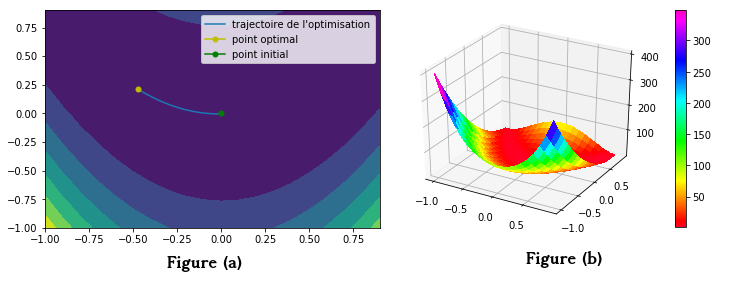
\includegraphics[width=0.8\textwidth]{f3.png}
 		\caption{Optimisation de la fonction $f(x)=100(x_1-x_2^2)^2+(1-x_1)^2$ pour $\epsilon=0.005$ et le nombre d'itération=100}
 	\end{center}
 \end{figure}
\end{enumerate}
\section{Régression logistique}
La régression logistique implémentée utilise la descente de gradient pour optimiser le log de vraisemblance. Nous allons effectuer quelques tests sur la base de données USPS (chiffres manuscrits) en choisissant à chaque fois uniquement deux chiffres. Pour commencer, nous considérons les chiffres 1 et 7 et différentes valeurs pour $\epsilon$. 
 \begin{figure}[H]
	\begin{center}
		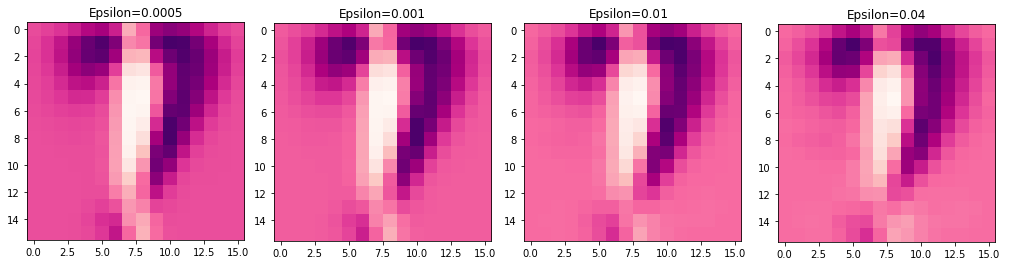
\includegraphics[width=0.8\textwidth]{reg_log.png}
		\caption{Les valeurs de poids de l'expérience 1Vs7 en fonction de  $\epsilon$}
	\end{center}
\end{figure}
\paragraph{}
Nous constatons que la valeur de $\epsilon$ qui nous approche le plus du résultat est de $\epsilon=0.01$ où nous pouvons voir très clairement les chiffres. Pour toutes les valeurs de $\epsilon=0.01$ citées dans la figure ci-dessous, le score obtenu était de 0.99 en apprentissage et de 0.98 en prédiction. 

\section{Bayes Naïf Vs Régression logistique }
\paragraph{}
Nous avons implémenté le classifier naïf de Bayes afin de comparer ses résultats avec les résultats fournis par la régression logistique. Dans tous les tests que nous avons effectués. Les résultats du classifier naïf de Bayes tournaient vers 0.93 en apprentissage et 0.87 en prédiction. Ce qui reste beaucoup moins satisfaisant que ce que nous obtenons avec la régression logistique qui quant à elle, elle ne retournait jamais des résultats au-dessous de 0.9 que ça soir en apprentissage ou en prédiction.
\chapter{Perceptron}
\section{Définition}
\paragraph{}
Nous étudions dans ce chapitre l'algorithme du Perceptron en se servant de la descente de gradient. Nous considérons comme fonctions de coûts deux fonctions soient: Les moindres carrés (MSE) et le hinge.
\section{Expérimentations}
\paragraph{}
Nous commençons notre étude par une comparaison de résultats entre les deux fonctions de coûts. Nous pouvons voir que qu'avec les deux méthodes, nous arrivons à séparer de façon acceptable les données. Or il n'est pas négligeable que le hinge a de meilleur résultat que le coût des moindres carrés. Cependant le hinge a comme résultat en apprentissage 0.994 et en test 0.989. Mais, le coût des moindres carrés a comme résultat en apprentissage et en prédiction 0.986.
\paragraph{}
Comme la fonction MSE représente une régression linéaire pour le perceptron, elle retourne un résultat moins bon que le hinge car elle pénalise quelques exemples qui basiquement sont bien classés mais éloignés de la droite séparatrice. Or, le hinge qui elle est bien adaptée au perceptron, elle cherche à corriger le vecteurs de poids à chaque itération uniquement lorsque la prédiction est fausse. 
 \begin{figure}[H]
	\begin{center}
		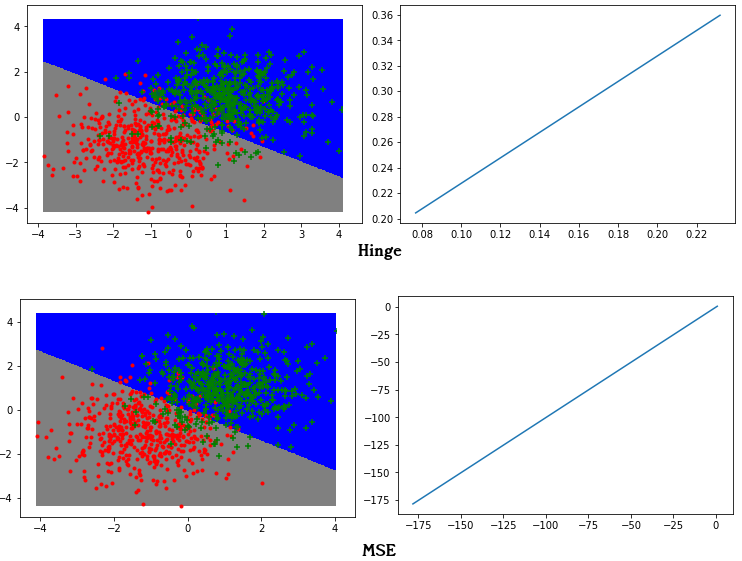
\includegraphics[width=0.6\textwidth]{hVSm.png}
		\caption{Perceptron avec différentes fonctions de coût avec $\epsilon=0.2$ et le nombre maximum d'itérations=200}
	\end{center}
\end{figure}
\paragraph{}
Nous avons effectué 
\subsection{Considération du biais}
\paragraph{}
Le biais permet de rendre le modèle plus expressif. Nous avons effectué quelques expériences pour voir ce que le biais pourrait rapporter à la précision du modèle.
\paragraph{}
Sur plusieurs exécutions données en minibatch, approximativement l'expérience sans biais à comme score 0.8 en apprentissage et en test. Cependant, lorsque nous considérons le biais nous n'obtenons jamais de score inférieur a 0.9.
 \begin{figure}[H]
	\begin{center}
		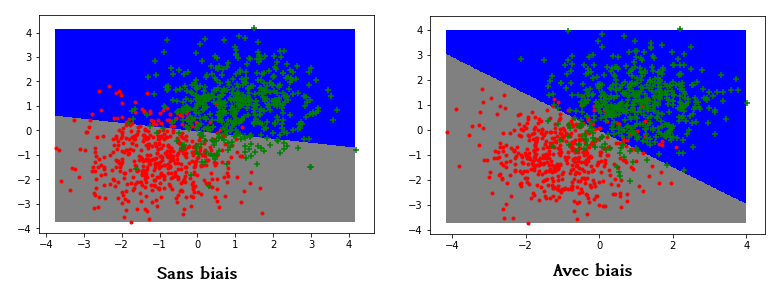
\includegraphics[width=0.8\textwidth]{sansbiaisVSbiais.png}
		\caption{L'impact du biais sur le perceptron avec $\epsilon=0.2$ et le nombre maximum d'itérations=200}
	\end{center}
\end{figure}

 
\subsection{Batch - MiniBatch - Stochastique}
Nous avons implémenté les trois variantes de l'algorithme: batch, miniBatch et stochastique. La variante qui est le plus rapide en convergence c'est Batch or son temps d'exécution est très coûteux comparant au stochastique qui ne considère qu'un exemple par itération. Cependant la variante stochastique reste moins bonne que le batch car nous ne prenons en compte qu'un exemple tiré aléatoirement pour corriger le vecteur des poids. Ceci produit le phénomène d'oscillations. Donc elle ne présente pas des résultats précis et satisfaisants comparant au batch.
\paragraph{}
Ensuite, comme relativement hybride, le minibatch se situe entre les deux autres variantes en terme de temps de calcul et en précision. Puisque en minibatch, nous ne considérons que des sous-ensembles de la base de donnée tirés de façon aléatoire.
 \begin{figure}[H]
	\begin{center}
		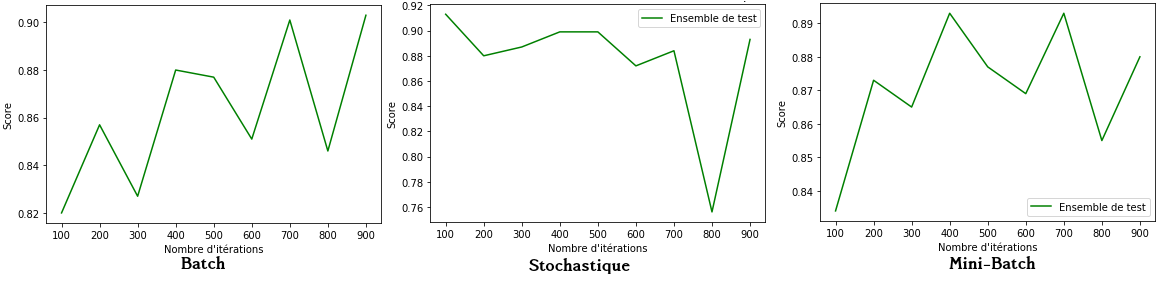
\includegraphics[width=0.9\textwidth]{variantes.png}
		\caption{Évaluation des variantes de l'algorithme du Perceptron en fonction du nombre d'itérations et avec $\epsilon=0.1$}
	\end{center}
\end{figure}
\subsection{Données USPS}
\paragraph{}
Reprenons les données USPS et sans considération du biais. Nous allons évaluer le perceptron sur différents ensembles de chiffres et analyser les courbes d'erreurs en apprentissage et en test en fonction du nombre d'itérations effectuées.
\paragraph{}
 \begin{figure}[H]
	\begin{center}
		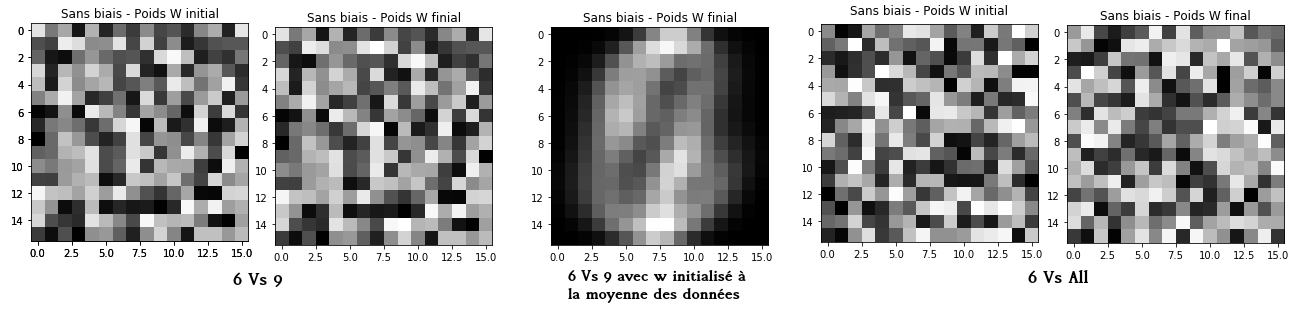
\includegraphics[width=0.8\textwidth]{6717.png}
		\caption{Visualisation de la matrice des poids sans biais avec $\epsilon=0.1$ et le nombre maximum d'itérations=1000}
	\end{center}
\end{figure}
Nous avons choisi les chiffres 6 et 9 dans cette expérience. Nous avons pris en compte l'initialisation du vecteur de poids. Premièrement nous l'avons initialisé de façon aléatoire. Les résultats n'étaient pas très satisfaisants comparant à la prise en compte des données. Deuxièmement, nous avons considéré ce dernier critère cité en initialisant le vecteurs de poids avec la moyenne des valeurs de la base de données. La figure ci-dessus montre clairement les chiffres 6 et 9 en tenant compte des données.
 \begin{figure}[H]
	\begin{center}
		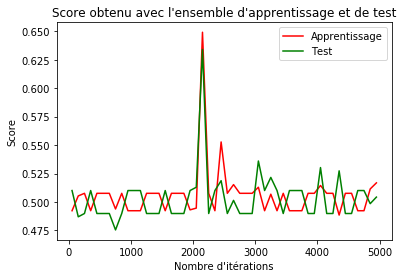
\includegraphics[width=0.4\textwidth]{69_steps.png}
		\caption{Les courbes d’erreurs en apprentissage et en test en fonction du nombre d’itérations.  avec $\epsilon=0.1$ }
	\end{center}
\end{figure}

\subsection{Projection polynomiale}
Nous avons effectué deux sortes de projection polynomiale:
\begin{enumerate}
	\item En rajoutant 3 dimensions à notre base de données: $x_1^2,x_2^2,x_1x_2$
	\item En remplaçant la base de données par: $x_1^2,x_2^2,\sqrt{x_1x_2}$
\end{enumerate}
 \begin{figure}[H]
	\begin{center}
		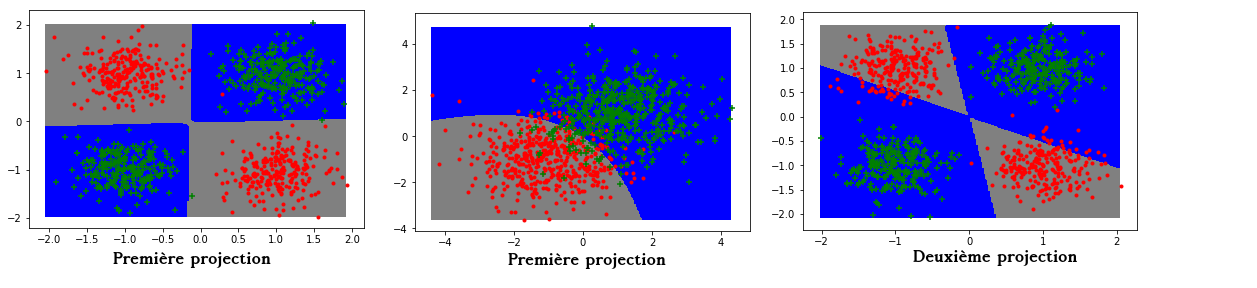
\includegraphics[width=0.9\textwidth]{proj.png}
		\caption{Perceptron avec différentes projections polynomiales avec $\epsilon=0.2$ et le nombre maximum d'itérations=1000}
	\end{center}
\end{figure}
\paragraph{}
Nous remarquons que le modèle tel construit a réussi à séparer les classes du XOR correctement. Nous pouvons dire que plus le nombre de dimensions que nous considérons lors de la projection est grand, plus nous garantissons de meilleures résultats. Par conséquent le nombre de dimensions rajouté affecte l'expressivité du modèle.
\subsection{Projection gaussienne}
\paragraph{}
Dans cette partie, nous considérons la projection gaussienne pour voir ce quelle peut rapporter à l'expressivité du modèle. L'expérience manipule des données générées aléatoirement et varie le nombre de points pour la base de projection. Nous avons effectué cette expérience pour les deux variantes d'algorithmes: minibatch et stochastique.  
 \begin{figure}[H]
	\begin{center}
		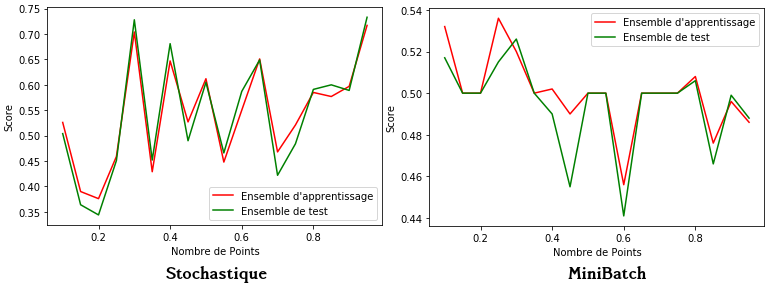
\includegraphics[width=0.9\textwidth]{gauss_nb.png}
		\caption{Projection gaussienne en fonction du nombre de points et des variantes du perceptron $\epsilon=0.2$ et le nombre maximum d'itérations=1000}
	\end{center}
\end{figure}
\paragraph{}
Nous constatons que lorsqu'il y a peu de données le minibatch a le meilleur score en apprentissage. Nous pouvons dire qu'une petite base de données n'est pas difficile à apprendre vu sa taille. Or, lorsqu'il s'agit d'une base de données très riche la courbe d'apprentissage se superpose approximativement sur celle de test et toutes les deux ont tendance à décroître car la généralisation devient vite difficile à cause du  très grand nombre de points dont nous disposons. Vers 0.5 Le modèle semble se stabiliser. Nous concluons qu'il vaut mieux une base de données de taille ni trop petite ni trop grande. 
\end{document}